\subsection{Induktive Ladung}\label{sec:energieuebertragung}

Der Dōjō wird mit Hilfe des Induktionsprinzips geladen. Der Ladeprozess wird gestartet, sobald der Dōjō auf die Ladestation gestellt wird. Beim Induktionsprinzip wird die Energie mithilfe von Spulen über eine kurze Distanz zwischen zwei Schaltungen transportiert. Die erste Schaltung wird Transceiver genannt und sendet die Energie. Sie besteht aus einem Pulsgenerator, mit welchem das LC-Glied gepulst wird. Sie macht den Hauptanteil einer solchen induktiven Ladeschaltung aus. Die zweite Schaltung wird Receiver genannt und empfängt die Energie. Sie besteht ebenfalls aus einem LC-Glied, hat jedoch zusätzlich einen Gleichrichter. Nachfolgend werden die Transceiver- und Receiverschaltung beschrieben, welche sich auf Abbildung \ref{fig:Tranceiver-Schaltung} beziehen.


\subsubsection*{Transceiver}
Als Pulsgenerator der Transceiver-Schaltung wird die Timer-Schaltung des NE555 verwendet, welcher mit 10V gespiesen wird. Diese Timer-Schaltung bietet den Vorteil, dass sie ohne grossen Aufwand zu erstellen und  einzustellen ist. Diese Eigenschaften haben diesen Timer-Baustein zum Standard IC für Zeitschaltungen gemacht. Der NE555 enthält eine monolithisch integrierte Zeitgeberschaltung, die sich aufgrund ihrer Eigenschaften als Taktgeber, Oszillator und für Zeitverzögerungen verwenden lässt. Der NE555 ist so universell einsetzbar, dass er als wichtigster integrierter Schaltkreis gilt. Das Funktionsprinzip beruht auf der Programmierung durch externe Komponenten. Das heisst, dass mithilfe von verschiedenen Verhältnissen der extern angeschlossenen Komponenten (bestehend aus Widerständen und Kondensatoren), die Pulsdauer, Frequenz und der Duty cycles eingestellt werden kann. Das dabei entstehende Pulssignal wird benutzt, um das LC-Glied zu pulsen, welches aus der Parallelschaltung unserer $14.9 \mu H$  Transceiverspule ($U\$1$) und $220 nF$ Kondensators $C_{3}$ besteht (Abbildung \ref{fig:Tranceiver-Schaltung}). Um dies zu ermöglichen wird dieses Glied an die Versorgungsspannung gehängt und in Serie dazu der Kollektor Anschluss eines $2N3055$ Leistungs NPN-Transistor. An dessen Emitter wird nun ein Niederohmiger Widerstand ($R_{4}$) auf GND gehängt. Dieser dient als Strombegrenzung, da die Spannung welche über ihm Abfällt von einem zweiten Transistor ($2N2222$) überwacht wird. Dieser 2N2222 Transistor wird zwischen dem Pulssignal, welches den $2N3055$ Leistungs-Transistor steuert, und GND gehängt. Wird nun der Strom und somit auch die Spannung über dem Widerstand $R_{4}$ zu hoch, so schliesst der 2N2222 Transistor das Pulssignal kurz. Der 2N3055 Leistungstransistor wird nicht mehr sauber durch gesteuert und der Strom wird begrenzt. Die Strombegrenzung ist von den verwendeten Komponenten des LC-Gliedes abhängig. Es ist darauf zu achten, welches der Beiden Elemente (LC-Glied/Leistungstransistor) weniger Strom verträgt. In diesem Fall ist dies die Spule, welche aufgrund ihrer geringen Baugrösse nur einen Strom von $0.6A$ verträgt. Würden grössere Spulen verwendet, so gilt spätestens bei einem Strom von $15A$ zu begrenzen, da dies die Belastungsgrenze für den $2N3055$ Leistungstransistor ist.   


\begin{figure}[H]
	\begin{center}
		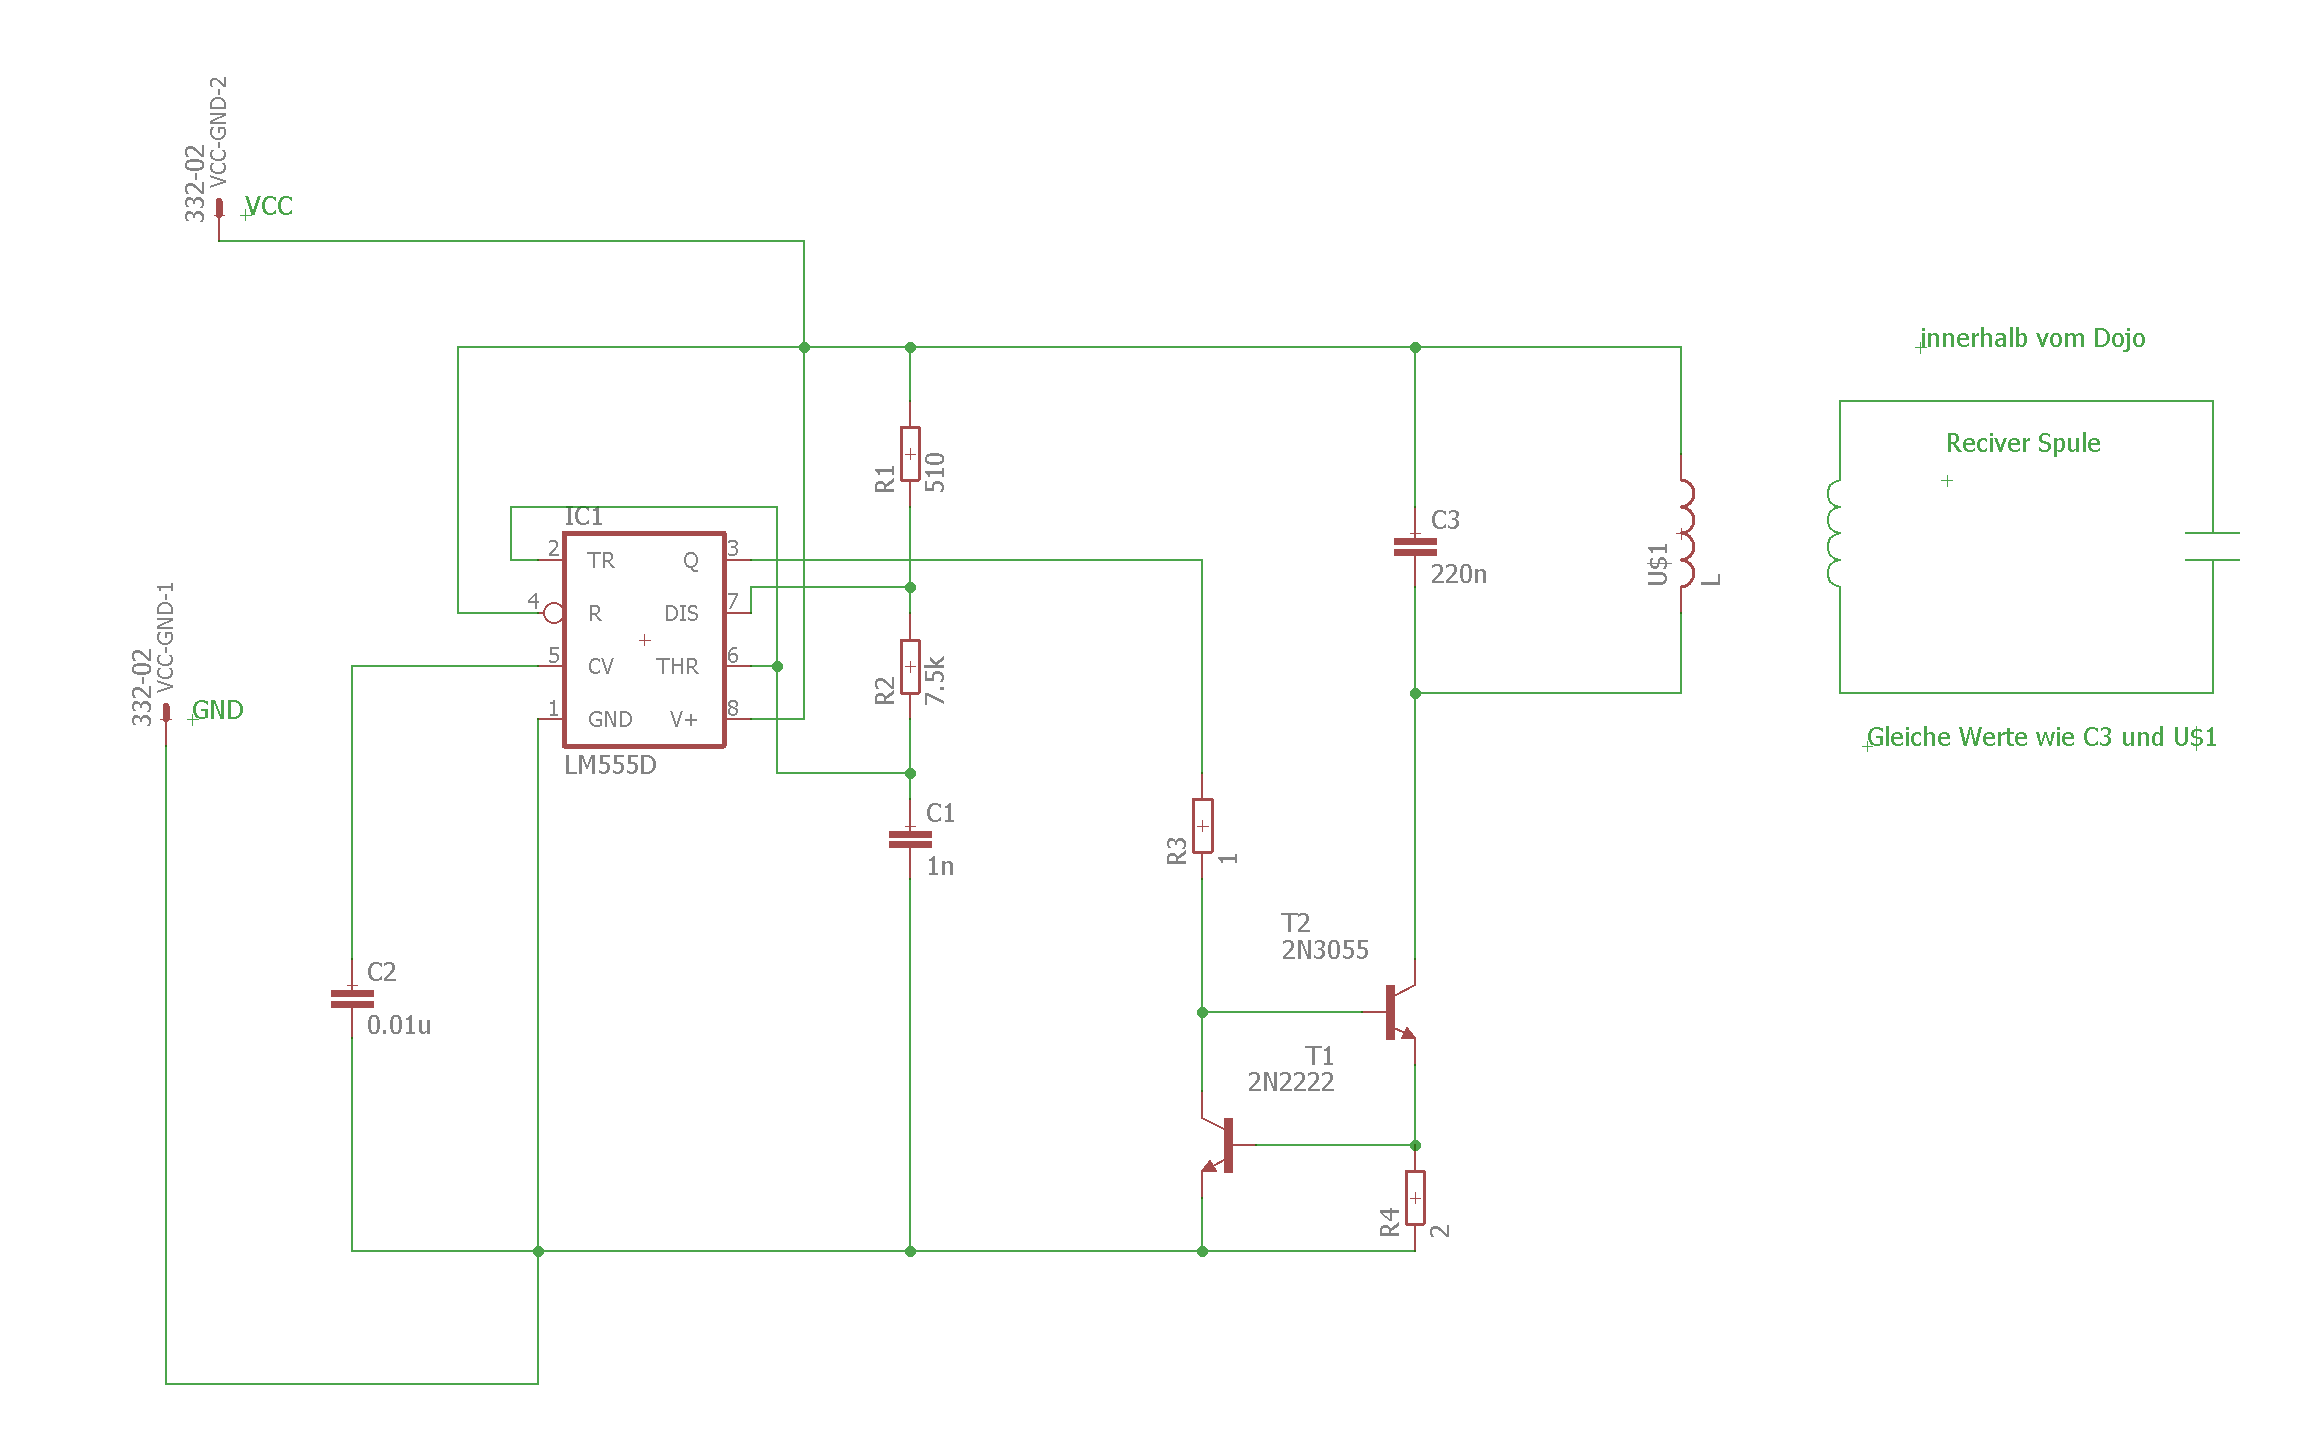
\includegraphics[width=160mm]{data/Tranceiver.png}
		\caption[Verwendete Timerschaltung als Pulsquelle]{Verwendete Timerschaltung als Pulsquelle} %picture caption
		\label{fig:Tranceiver-Schaltung}
	\end{center}
\end{figure}
 
Das Pulssignal selber muss verschiedene Kriterien erfüllen. Zum einen sollte der Duty Cycle so nahe wie möglich an $50\%$ sein. Um dies zu erreichen muss $R2 >> R1$ gelten. Das andere Kriterium ist die Erreichung der Resonanzfrequenz ($f_{res}$) des LC-Gliedes. Diese wird wie folgt aus den Komponenten des LC-Gliedes berechnet.

\begin{equation}\label{eq:Resonanz}
f_{res}=\frac{\sqrt{L\cdot C}}{2\cdot \pi}
\end{equation}

Die ideale Frequenz würde $93kHz$ betragen. Jedoch musste diese auf $79kHz$ angepasst werden da die nachfolgende Ladeschaltung nicht ideal dimensioniert wurde. Genaueres dazu ist in der Validierung der Hardware zu finden.
Um das Pulssignal theoretisch optimal einzustellen, können folgende Richtlinien betrachtet werden:

\begin{description}
	\item [$\cdot$ C] beeinflusst die Zeiten (Frequenz/High-Time/Low-Time)
	\item [$\cdot$ R$_{1}$] beeinflusst die High-Time, lässt jedoch die Low-Time unverändert.
	\item [$\cdot$ R$_{2}$ ] beeinflusst die High- und Low-Time und beeinflusst somit den Duty Cycle.
\end{description}


Die verwendeten Komponenten $C$, $R_{1}$ und $R_{2}$, welche in der Abbildung  \ref{fig:Tranceiver-Schaltung} rechts vom Timer Baustein ($LM555D$) zu sehen sind, wurden durch nachfolgende Formeln \ref{eq:Timerf} bis \ref{eq:TimerR2} berechnet. 


Zuerst wollen wir unsere ideale Taktfrequenz berechnen. Dabei werden wir zuerst einen Kondensator auswählen. Da dieser die Zeit massgebend beeinflusst, ist darauf zu achten, dass dieser eher klein zu wählen ist, da sonst die Widerstandswerte ins unermässliche gehen.
\begin{equation}\label{eq:Timerf}
f= \dfrac{1}{T}= \dfrac{1.44}{((R_{1} + 2 \cdot R_{2})\cdot C)}
\end{equation}

Nun bleiben noch die Widerstände zu bestimmen. Wir wollen einen Duty Cycle von ca $50%$. Das heisst, dass Low- und High-Time beinahe identisch sind. Daraus lässt sich schliessen, dass $R1$ vernachlässigbar klein ist. Dieser könnte allenfalls sogar als $0$ angenommen werden, jedoch lässt sich so nicht jede beliebige Frequenz einstellen mit den vorhandenen Widerstandswerten für $R2$. Dieser müsste aus mehreren Widerständen zusammengesetzt werden. Daher entschieden wir uns dafür einen kleinen Wert für $R1$ anzunehmen, was sich beim Duty-Cycle kaum bemerkbar machte.
\begin{equation}\label{eq:TimerTL}
LowTime= 0.693 \cdot R_{2} \cdot C
\end{equation}
\begin{equation}\label{eq:TimerTH}
HighTime= 0.693 \cdot (R_{1} + R_{2}) \cdot C
\end{equation}
\begin{equation}\label{eq:TimerDC}
D = DutyCycle = \dfrac{R_{1} + R_{2}}{R_{1} + 2 \cdot R_{2}}
\end{equation}

Somit wären alle Komponenten bestummen. Möchte man eine andere Vorgehensweise wählen, so stünden noch die folgenden Formeln \ref{eq:TimerR1} und \ref{eq:TimerR2} zur verfügung.
\begin{equation}\label{eq:TimerR1}
R1 = 1.44 \cdot \left( \dfrac{2 \cdot D - 1}{f \cdot C} \right)
\end{equation}
\begin{equation}\label{eq:TimerR2}
R2 = 1.44 \cdot \left( \dfrac{1-D}{f \cdot C} \right)
\end{equation} 


Für die Berechnung der effektiven Werte, müssen die ersten Werte angenommen werden. Deshalb lohnt es sich einen Wert für den Kondensator $C$ anzunehmen, da dessen verfügbare Werte durch die E-Reihen begrenzt sind. Es ist zu erwähnen, dass es sich bei den bereits eingefügten Zahlenwerten um Konstanten handelt, welche in jedem handelsüblichen Datenblatt eines $555$ Timer-Bausteins zu finden sind. Unsere Berechnungen ergaben für die angepasste Tranceiver Schaltung mit einer verringerten Taktfrequenz von $79.12 kHz$ folgende Werte:

\begin{center}
$C_{1}$ = $1nF$\\
$R_{1}$ = $200\Omega$\\
$R_{2}$ = $9k\Omega$\\
\end{center}

Diese Bauteile sind in Abbildung \ref{fig:Tranceiver-Schaltung} zu sehen, wobei die neu berechneten Werte der Widerstände nicht mehr mit den ursprünglichen Werten im Schema korrelieren.
Nach dem die Werte berechnet wurden, können die einzelnen Komponenten ausgewählt und implementiert werden. Dabei gilt es zu beachten, dass minimale Abweichungen bereits zu einer Änderung der Frequenz, Pulsdauer und Duty-Cycle des Pulssignales führen.

\subsubsection*{Receiver}
Der Receiver besteht primär aus einem LC-Glied und einem Gleichrichter. Speziell ist, dass bei der Tranceiverschaltung das selbe LC-Glied verwendet wurde wie bei der Receiverschaltung. (Wie in Abbildung \ref{fig:Tranceiver-Schaltung} rechts oben zu sehen besteht das LC-Glied aus der Flachspule L mit einem Wert von $14.9uH$ und einem Koppelkondensator $C_{3}$ mit $220nF$). Dies wurde aus dem Grund gewählt, weil das Energiefeld bei einem identischen LC-Glieder Paar am effektivsten ausgenutzt werden kann. Das L-Glied (Flachspule) lässt sich mit einer Dimension von $\o 15mm$ Durchmesser und $0.2mm$ Höhe gut im inneren des Dōjō’s platzieren. Die Positionierung findet am Boden statt, da dieser eben ist und somit als Standfläche für den Dōjō genutzt wird. Somit kann dieser schlussendlich in der Ladestation platziert werden, ohne davon zu rollen. Die hochfrequente Wechselspannung welche nun am Dōjō anliegt, muss für die Speisung der Batterie noch gleichgerichtet werden. Hierbei können beliebige Dioden verwendet und zu einem Brückengleichrichter verschaltet werden. Wir entschieden uns für Schotky-Dioden, da diese mit einer Durchlassspannung von $0.2V$ die übertragene Spannung nur leicht abschwächen. Anschliessend wird die Ladeschaltung gespiesen, welche den gesamten Ladeprozess des Akkus übernimmt. Einen Einblick in diesen Ladeprozess gibt nachfolgendes Kapitel.

